\chapter{Problème des règles de Golomb}

\epigraph{\textit{``Mathematics is the art of giving the same name to different things.''}}{--- Henri Poincaré}

\section{Définition formelle, notations et contraintes}

\subsection{Définition d'une règle de Golomb}

\begin{definition}[Règle de Golomb]
Une \textbf{règle de Golomb} d'ordre $n$ est un ensemble de $n$ entiers positifs distincts $G = \{m_0, m_1, \ldots, m_{n-1}\}$ appelés \textit{marques}, avec la convention $m_0 = 0 < m_1 < m_2 < \cdots < m_{n-1}$, tel que toutes les différences $m_j - m_i$ pour $i < j$ sont distinctes.
\end{definition}

Formellement, la \textbf{propriété de Golomb} s'exprime :
\begin{equation}
\forall (i,j,k,l) \in \{0, \ldots, n-1\}^4 \text{ avec } i < j \text{ et } k < l : \quad (i,j) \neq (k,l) \Rightarrow m_j - m_i \neq m_l - m_k
\end{equation}

\subsection{Notations}

Nous adoptons les notations suivantes tout au long de ce rapport :

\begin{table}[H]
\centering
\begin{tabular}{cl}
\toprule
\textbf{Notation} & \textbf{Signification} \\
\midrule
$n$ & Ordre de la règle (nombre de marques) \\
$G_n$ & Règle de Golomb d'ordre $n$ \\
$m_i$ & Position de la $i$-ème marque ($m_0 = 0$) \\
$L(G_n)$ & Longueur de la règle $G_n$, définie par $L(G_n) = m_{n-1}$ \\
$D(G_n)$ & Ensemble des différences : $D(G_n) = \{m_j - m_i : 0 \leq i < j \leq n-1\}$ \\
$OGR(n)$ & Règle de Golomb optimale d'ordre $n$ \\
$L^*(n)$ & Longueur minimale d'une règle de Golomb d'ordre $n$ \\
\bottomrule
\end{tabular}
\caption{Notations utilisées pour les règles de Golomb}
\label{tab:notations}
\end{table}

\subsection{Représentation graphique}

Une règle de Golomb peut être visualisée comme une règle graduée où seules certaines positions sont marquées. La figure \ref{fig:golomb_example} illustre la règle optimale d'ordre 4 : $G_4 = \{0, 1, 4, 6\}$.

\begin{figure}[H]
\centering
\begin{tikzpicture}[scale=0.8]
    % Règle principale
    \draw[thick] (0,0) -- (12,0);

    % Graduations
    \foreach \x in {0,1,...,12} {
        \draw (\x,-0.1) -- (\x,0.1);
        \node[below] at (\x,-0.2) {\tiny \x};
    }

    % Marques de Golomb (positions 0, 1, 4, 6)
    \foreach \x/\label in {0/m_0, 2/m_1, 8/m_2, 12/m_3} {
        \draw[fill=burgundy, burgundy] (\x,-0.3) -- (\x,0.5);
        \draw[fill=burgundy] (\x,0.5) circle (0.15);
    }

    % Annotations des positions
    \node[above] at (0,0.7) {$0$};
    \node[above] at (2,0.7) {$1$};
    \node[above] at (8,0.7) {$4$};
    \node[above] at (12,0.7) {$6$};

    % Différences (arcs)
    \draw[<->, gold, thick] (0,-0.8) -- (2,-0.8) node[midway, below] {\small 1};
    \draw[<->, gold, thick] (2,-1.4) -- (8,-1.4) node[midway, below] {\small 3};
    \draw[<->, gold, thick] (8,-0.8) -- (12,-0.8) node[midway, below] {\small 2};
    \draw[<->, burgundy!70, thick] (0,-2.0) -- (8,-2.0) node[midway, below] {\small 4};
    \draw[<->, burgundy!70, thick] (2,-2.6) -- (12,-2.6) node[midway, below] {\small 5};
    \draw[<->, burgundy!50, thick] (0,-3.2) -- (12,-3.2) node[midway, below] {\small 6};
\end{tikzpicture}
\caption{Règle de Golomb optimale d'ordre 4 : $G_4 = \{0, 1, 4, 6\}$. Les 6 différences (1, 2, 3, 4, 5, 6) sont toutes distinctes.}
\label{fig:golomb_example}
\end{figure}

\subsection{Nombre de différences}

Pour une règle d'ordre $n$, le nombre de paires de marques distinctes est :
\begin{equation}
|D(G_n)| = \binom{n}{2} = \frac{n(n-1)}{2}
\end{equation}

Ce nombre correspond au nombre de différences à vérifier pour s'assurer de l'unicité. Par exemple :
\begin{itemize}
    \item $n = 4$ marques $\Rightarrow$ 6 différences
    \item $n = 7$ marques $\Rightarrow$ 21 différences
    \item $n = 13$ marques $\Rightarrow$ 78 différences
\end{itemize}

\subsection{Contraintes structurelles}

\begin{theorem}[Borne inférieure triviale]
Pour toute règle de Golomb d'ordre $n$, la longueur vérifie :
\begin{equation}
L(G_n) \geq \frac{n(n-1)}{2}
\end{equation}
\end{theorem}

\begin{proof}
Les $\binom{n}{2}$ différences doivent être distinctes et positives. La plus petite configuration possible serait que ces différences soient exactement $\{1, 2, 3, \ldots, \binom{n}{2}\}$. La plus grande différence, qui est la longueur de la règle, est donc au moins $\binom{n}{2}$.
\end{proof}

\begin{remark}
Une règle atteignant cette borne inférieure est dite \textbf{parfaite}. Les règles parfaites sont rares : elles n'existent que pour $n \in \{1, 2, 3, 4\}$.
\end{remark}

\section{Critère d'optimalité}

\subsection{Définition de l'optimalité}

\begin{definition}[Règle de Golomb optimale]
Une règle de Golomb $G_n^*$ d'ordre $n$ est dite \textbf{optimale} si sa longueur est minimale parmi toutes les règles de Golomb du même ordre :
\begin{equation}
L(G_n^*) = L^*(n) = \min\{L(G_n) : G_n \text{ est une règle de Golomb d'ordre } n\}
\end{equation}
\end{definition}

Le problème de recherche de la règle de Golomb optimale (\textit{Optimal Golomb Ruler}, OGR) est un problème d'optimisation combinatoire :

\begin{important}{Problème OGR}
\textbf{Entrée :} Un entier $n \geq 2$. \\
\textbf{Sortie :} Une règle de Golomb $G_n^* = \{0, m_1, \ldots, m_{n-1}\}$ de longueur minimale $L^*(n)$.
\end{important}

\subsection{Complexité du problème}

Le problème OGR est \textbf{NP-difficile}. Cela implique qu'aucun algorithme polynomial n'est connu pour le résoudre. En pratique, la recherche exhaustive de l'optimum requiert un temps exponentiel en $n$.

L'espace de recherche peut être estimé comme suit : pour une règle d'ordre $n$ avec longueur maximale $L_{max}$, le nombre de configurations possibles est de l'ordre de $\binom{L_{max}}{n-1}$, qui croît exponentiellement.

\begin{figure}[H]
\centering
\begin{tikzpicture}[scale=0.9]
    \begin{axis}[
        xlabel={Ordre $n$},
        ylabel={Temps relatif (échelle log)},
        ymode=log,
        grid=major,
        width=10cm,
        height=6cm,
        legend pos=north west,
        xtick={4,5,6,7,8,9,10,11,12,13},
    ]
    \addplot[mark=*, burgundy, thick] coordinates {
        (4, 0.001)
        (5, 0.002)
        (6, 0.01)
        (7, 0.05)
        (8, 0.3)
        (9, 2)
        (10, 15)
        (11, 150)
        (12, 1500)
        (13, 20000)
    };
    \addlegendentry{Temps de calcul}
    \end{axis}
\end{tikzpicture}
\caption{Croissance exponentielle du temps de calcul en fonction de l'ordre $n$}
\label{fig:complexity}
\end{figure}

\subsection{Équivalence et symétrie}

Deux règles de Golomb sont dites \textbf{équivalentes} si l'une peut être obtenue à partir de l'autre par :
\begin{itemize}
    \item \textbf{Translation} : ajout d'une constante à toutes les marques (éliminée par convention $m_0 = 0$) ;
    \item \textbf{Réflexion} : transformation $m_i \mapsto L - m_{n-1-i}$, qui inverse l'ordre des marques.
\end{itemize}

\begin{example}
Les règles $\{0, 1, 4, 6\}$ et $\{0, 2, 5, 6\}$ sont équivalentes par réflexion :
\[
\{0, 1, 4, 6\} \xrightarrow{\text{réflexion}} \{6-6, 6-4, 6-1, 6-0\} = \{0, 2, 5, 6\}
\]
\end{example}

Pour éviter les redondances, on impose souvent la convention $m_1 < L - m_{n-2}$, ce qui sélectionne une forme canonique parmi les deux équivalentes.

\section{Vérification d'une solution}

\subsection{Algorithme de vérification}

La vérification qu'un ensemble de marques forme bien une règle de Golomb consiste à s'assurer que toutes les différences sont distinctes. L'algorithme \ref{alg:verify} présente cette procédure.

\begin{algorithm}[H]
\caption{Vérification d'une règle de Golomb}
\label{alg:verify}
\begin{algorithmic}[1]
\Require Ensemble de marques $M = \{m_0, m_1, \ldots, m_{n-1}\}$ trié
\Ensure \texttt{true} si $M$ est une règle de Golomb, \texttt{false} sinon
\State $seen \gets \emptyset$ \Comment{Ensemble des différences vues}
\For{$i \gets 0$ \textbf{to} $n-2$}
    \For{$j \gets i+1$ \textbf{to} $n-1$}
        \State $d \gets m_j - m_i$
        \If{$d \in seen$}
            \State \Return \texttt{false} \Comment{Différence en double}
        \EndIf
        \State $seen \gets seen \cup \{d\}$
    \EndFor
\EndFor
\State \Return \texttt{true}
\end{algorithmic}
\end{algorithm}

\subsection{Complexité de la vérification}

\begin{itemize}
    \item \textbf{Approche naïve} (avec tableau ou ensemble) : $O(n^2)$ comparaisons, chaque insertion/recherche dans un ensemble haché étant $O(1)$ en moyenne.
    \item \textbf{Approche par bitset} : en utilisant un vecteur de bits indexé par les différences, la vérification reste $O(n^2)$ mais avec des opérations très rapides (accès mémoire contigus).
\end{itemize}

\subsection{Implémentation avec bitset}

Dans notre implémentation, nous utilisons un \texttt{bitset} pour représenter les différences déjà vues. Cette structure permet des opérations en $O(1)$ pour le test et le marquage :

\begin{lstlisting}[language=C++, caption={Vérification avec bitset en C++}]
static inline bool isValid(const std::vector<int>& marks) {
    std::bitset<MAX_DIFF> seen;
    const size_t size = marks.size();

    for (size_t i = 0; i < size; ++i) {
        const int mi = marks[i];
        for (size_t j = i + 1; j < size; ++j) {
            const int d = marks[j] - mi;
            if (d >= MAX_DIFF) return false;
            if (seen[d]) return false;  // Collision!
            seen.set(d);
        }
    }
    return true;
}
\end{lstlisting}

\subsection{Optimisation par décalage de bits}

Une optimisation clé de notre implémentation consiste à calculer \textit{toutes} les nouvelles différences en une seule opération de décalage (\textit{shift}). Cette technique, détaillée au chapitre 4, permet de passer d'une complexité $O(k)$ par marque ajoutée à $O(1)$ :

\begin{figure}[H]
\centering
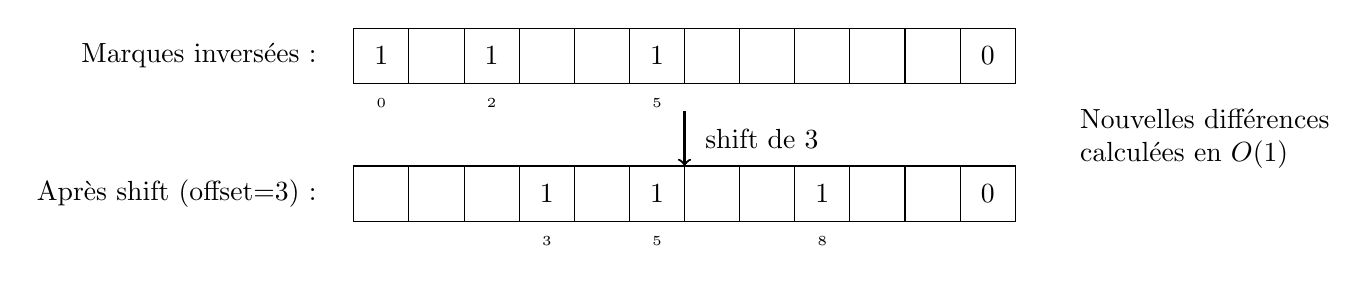
\begin{tikzpicture}[scale=0.7]
    % Bitset des marques inversées
    \node[anchor=east] at (-0.5, 2) {Marques inversées :};
    \draw (0,1.5) rectangle (12,2.5);
    \foreach \x/\val in {0/1, 2/1, 5/1, 11/0} {
        \node at (\x+0.5, 2) {\val};
    }
    \foreach \x in {0,1,...,11} {
        \draw (\x,1.5) -- (\x,2.5);
    }
    \node[below] at (0.5, 1.4) {\tiny 0};
    \node[below] at (2.5, 1.4) {\tiny 2};
    \node[below] at (5.5, 1.4) {\tiny 5};

    % Flèche
    \draw[->, thick] (6, 1) -- (6, 0);
    \node[right] at (6.2, 0.5) {shift de 3};

    % Bitset après décalage
    \node[anchor=east] at (-0.5, -0.5) {Après shift (offset=3) :};
    \draw (0,-1) rectangle (12,0);
    \foreach \x/\val in {3/1, 5/1, 8/1, 11/0} {
        \node at (\x+0.5, -0.5) {\val};
    }
    \foreach \x in {0,1,...,11} {
        \draw (\x,-1) -- (\x,0);
    }
    \node[below] at (3.5, -1.1) {\tiny 3};
    \node[below] at (5.5, -1.1) {\tiny 5};
    \node[below] at (8.5, -1.1) {\tiny 8};

    % Explication
    \node[align=left, anchor=west] at (13, 0.5) {Nouvelles différences\\calculées en $O(1)$};
\end{tikzpicture}
\caption{Calcul des différences par décalage de bits}
\label{fig:bitshift}
\end{figure}

\section{Résultats optimaux connus}

\subsection{Historique et méthodes de découverte}

Les règles de Golomb optimales ont été découvertes progressivement :
\begin{itemize}
    \item Les petites valeurs ($n \leq 11$) ont été trouvées par des méthodes exhaustives classiques ;
    \item Les valeurs plus grandes ($n \geq 12$) ont nécessité des projets de calcul distribué comme \textit{distributed.net} et des années de calcul ;
    \item La règle optimale pour $n = 27$ (longueur 553) a été prouvée en 2014 après plus de 6 ans de calcul distribué.
\end{itemize}

\subsection{Table des résultats optimaux}

Le tableau \ref{tab:optimal_results} présente les règles de Golomb optimales connues jusqu'à $n = 14$, qui servent de référence pour valider notre implémentation.

\begin{table}[H]
\centering
\begin{tabular}{ccc}
\toprule
\textbf{Ordre $n$} & \textbf{Longueur $L^*(n)$} & \textbf{Règle optimale} \\
\midrule
2 & 1 & $\{0, 1\}$ \\
3 & 3 & $\{0, 1, 3\}$ \\
4 & 6 & $\{0, 1, 4, 6\}$ \\
5 & 11 & $\{0, 1, 4, 9, 11\}$ \\
6 & 17 & $\{0, 1, 4, 10, 12, 17\}$ \\
7 & 25 & $\{0, 1, 4, 10, 18, 23, 25\}$ \\
8 & 34 & $\{0, 1, 4, 9, 15, 22, 32, 34\}$ \\
9 & 44 & $\{0, 1, 5, 12, 25, 27, 35, 41, 44\}$ \\
10 & 55 & $\{0, 1, 6, 10, 23, 26, 34, 41, 53, 55\}$ \\
11 & 72 & $\{0, 1, 4, 13, 28, 33, 47, 54, 64, 70, 72\}$ \\
12 & 85 & $\{0, 2, 6, 24, 29, 40, 43, 55, 68, 75, 76, 85\}$ \\
13 & 106 & $\{0, 2, 5, 25, 37, 43, 59, 70, 85, 89, 98, 99, 106\}$ \\
14 & 127 & $\{0, 4, 6, 20, 35, 52, 59, 77, 78, 86, 89, 99, 122, 127\}$ \\
\bottomrule
\end{tabular}
\caption{Règles de Golomb optimales pour $n = 2$ à $14$}
\label{tab:optimal_results}
\end{table}

\subsection{Observations sur les résultats}

\begin{enumerate}
    \item \textbf{Règles parfaites} : Pour $n \leq 4$, $L^*(n) = \binom{n}{2}$ (borne inférieure atteinte). Au-delà, les règles ne sont plus parfaites.

    \item \textbf{Croissance} : La longueur optimale croît approximativement comme $O(n^2)$, mais le coefficient multiplicatif augmente avec $n$.

    \item \textbf{Non-unicité} : Il peut exister plusieurs règles optimales distinctes (non équivalentes) pour un même ordre. Par exemple, pour $n = 11$, il existe plusieurs règles de longueur 72.
\end{enumerate}

\begin{figure}[H]
\centering
\begin{tikzpicture}[scale=0.8]
    \begin{axis}[
        xlabel={Ordre $n$},
        ylabel={Longueur optimale $L^*(n)$},
        grid=major,
        width=12cm,
        height=7cm,
        legend pos=north west,
        xtick={2,3,4,5,6,7,8,9,10,11,12,13,14},
    ]
    % Longueur optimale
    \addplot[mark=*, burgundy, thick] coordinates {
        (2, 1) (3, 3) (4, 6) (5, 11) (6, 17) (7, 25)
        (8, 34) (9, 44) (10, 55) (11, 72) (12, 85) (13, 106) (14, 127)
    };
    \addlegendentry{$L^*(n)$}

    % Borne inférieure
    \addplot[mark=square*, gold, dashed, thick] coordinates {
        (2, 1) (3, 3) (4, 6) (5, 10) (6, 15) (7, 21)
        (8, 28) (9, 36) (10, 45) (11, 55) (12, 66) (13, 78) (14, 91)
    };
    \addlegendentry{$\binom{n}{2}$ (borne inf.)}
    \end{axis}
\end{tikzpicture}
\caption{Comparaison entre longueur optimale et borne inférieure théorique}
\label{fig:optimal_vs_bound}
\end{figure}

\subsection{Validation de l'implémentation}

Ces résultats servent de \textit{ground truth} pour valider notre implémentation. Une implémentation correcte doit :
\begin{enumerate}
    \item Trouver exactement la longueur optimale $L^*(n)$ pour chaque ordre testé ;
    \item Retourner une règle valide (toutes les différences distinctes) ;
    \item La règle retournée peut différer de celles listées (équivalence ou autre optimal).
\end{enumerate}

\begin{defi}{Critère de validation}
L'implémentation est considérée \textbf{correcte} si et seulement si, pour tout $n$ testé :
\begin{enumerate}
    \item $L_{trouvée}(n) = L^*(n)$
    \item \texttt{isValid}$(G_{trouvée}) = $ \texttt{true}
\end{enumerate}
\end{defi}
